\chapter{Assignment: Model Explanation}
\label{hw:model-explanation}

\newthought{Understanding the model is essential for decision-making.} We are back to FTO3 data set. We have already built several models and evaluated their performance. But for reaching any kind of decisions, it is important to understand the model - what it does, which features are important, and in what way. We will continue working with the mean batch data.

\begin{figure}[h]
  \centering
  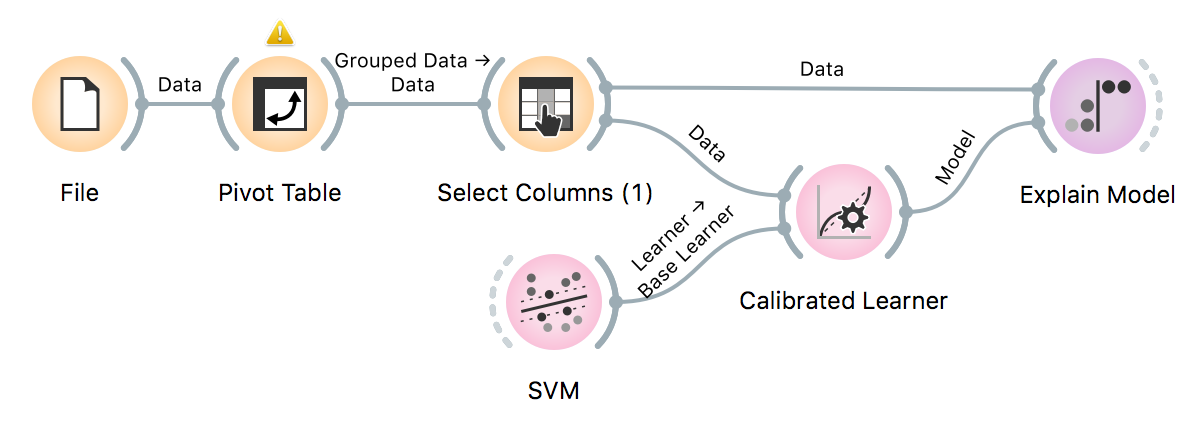
\includegraphics[width=\linewidth]{model-explanation.png}%
  \caption{$\;$}
  \label{fig:wf1}
\end{figure}

\begin{enumerate}
    \item What is the first thing you notice about the model? Hint: look at the distribution of the data.
    \item What are the top three attributes of the model? How are they interpreted?
    \item What is the main production decision that you can make after observing the model?
\end{enumerate}
